% 菲涅尔公式
%10 min

\begin{figure}[h]
\centering
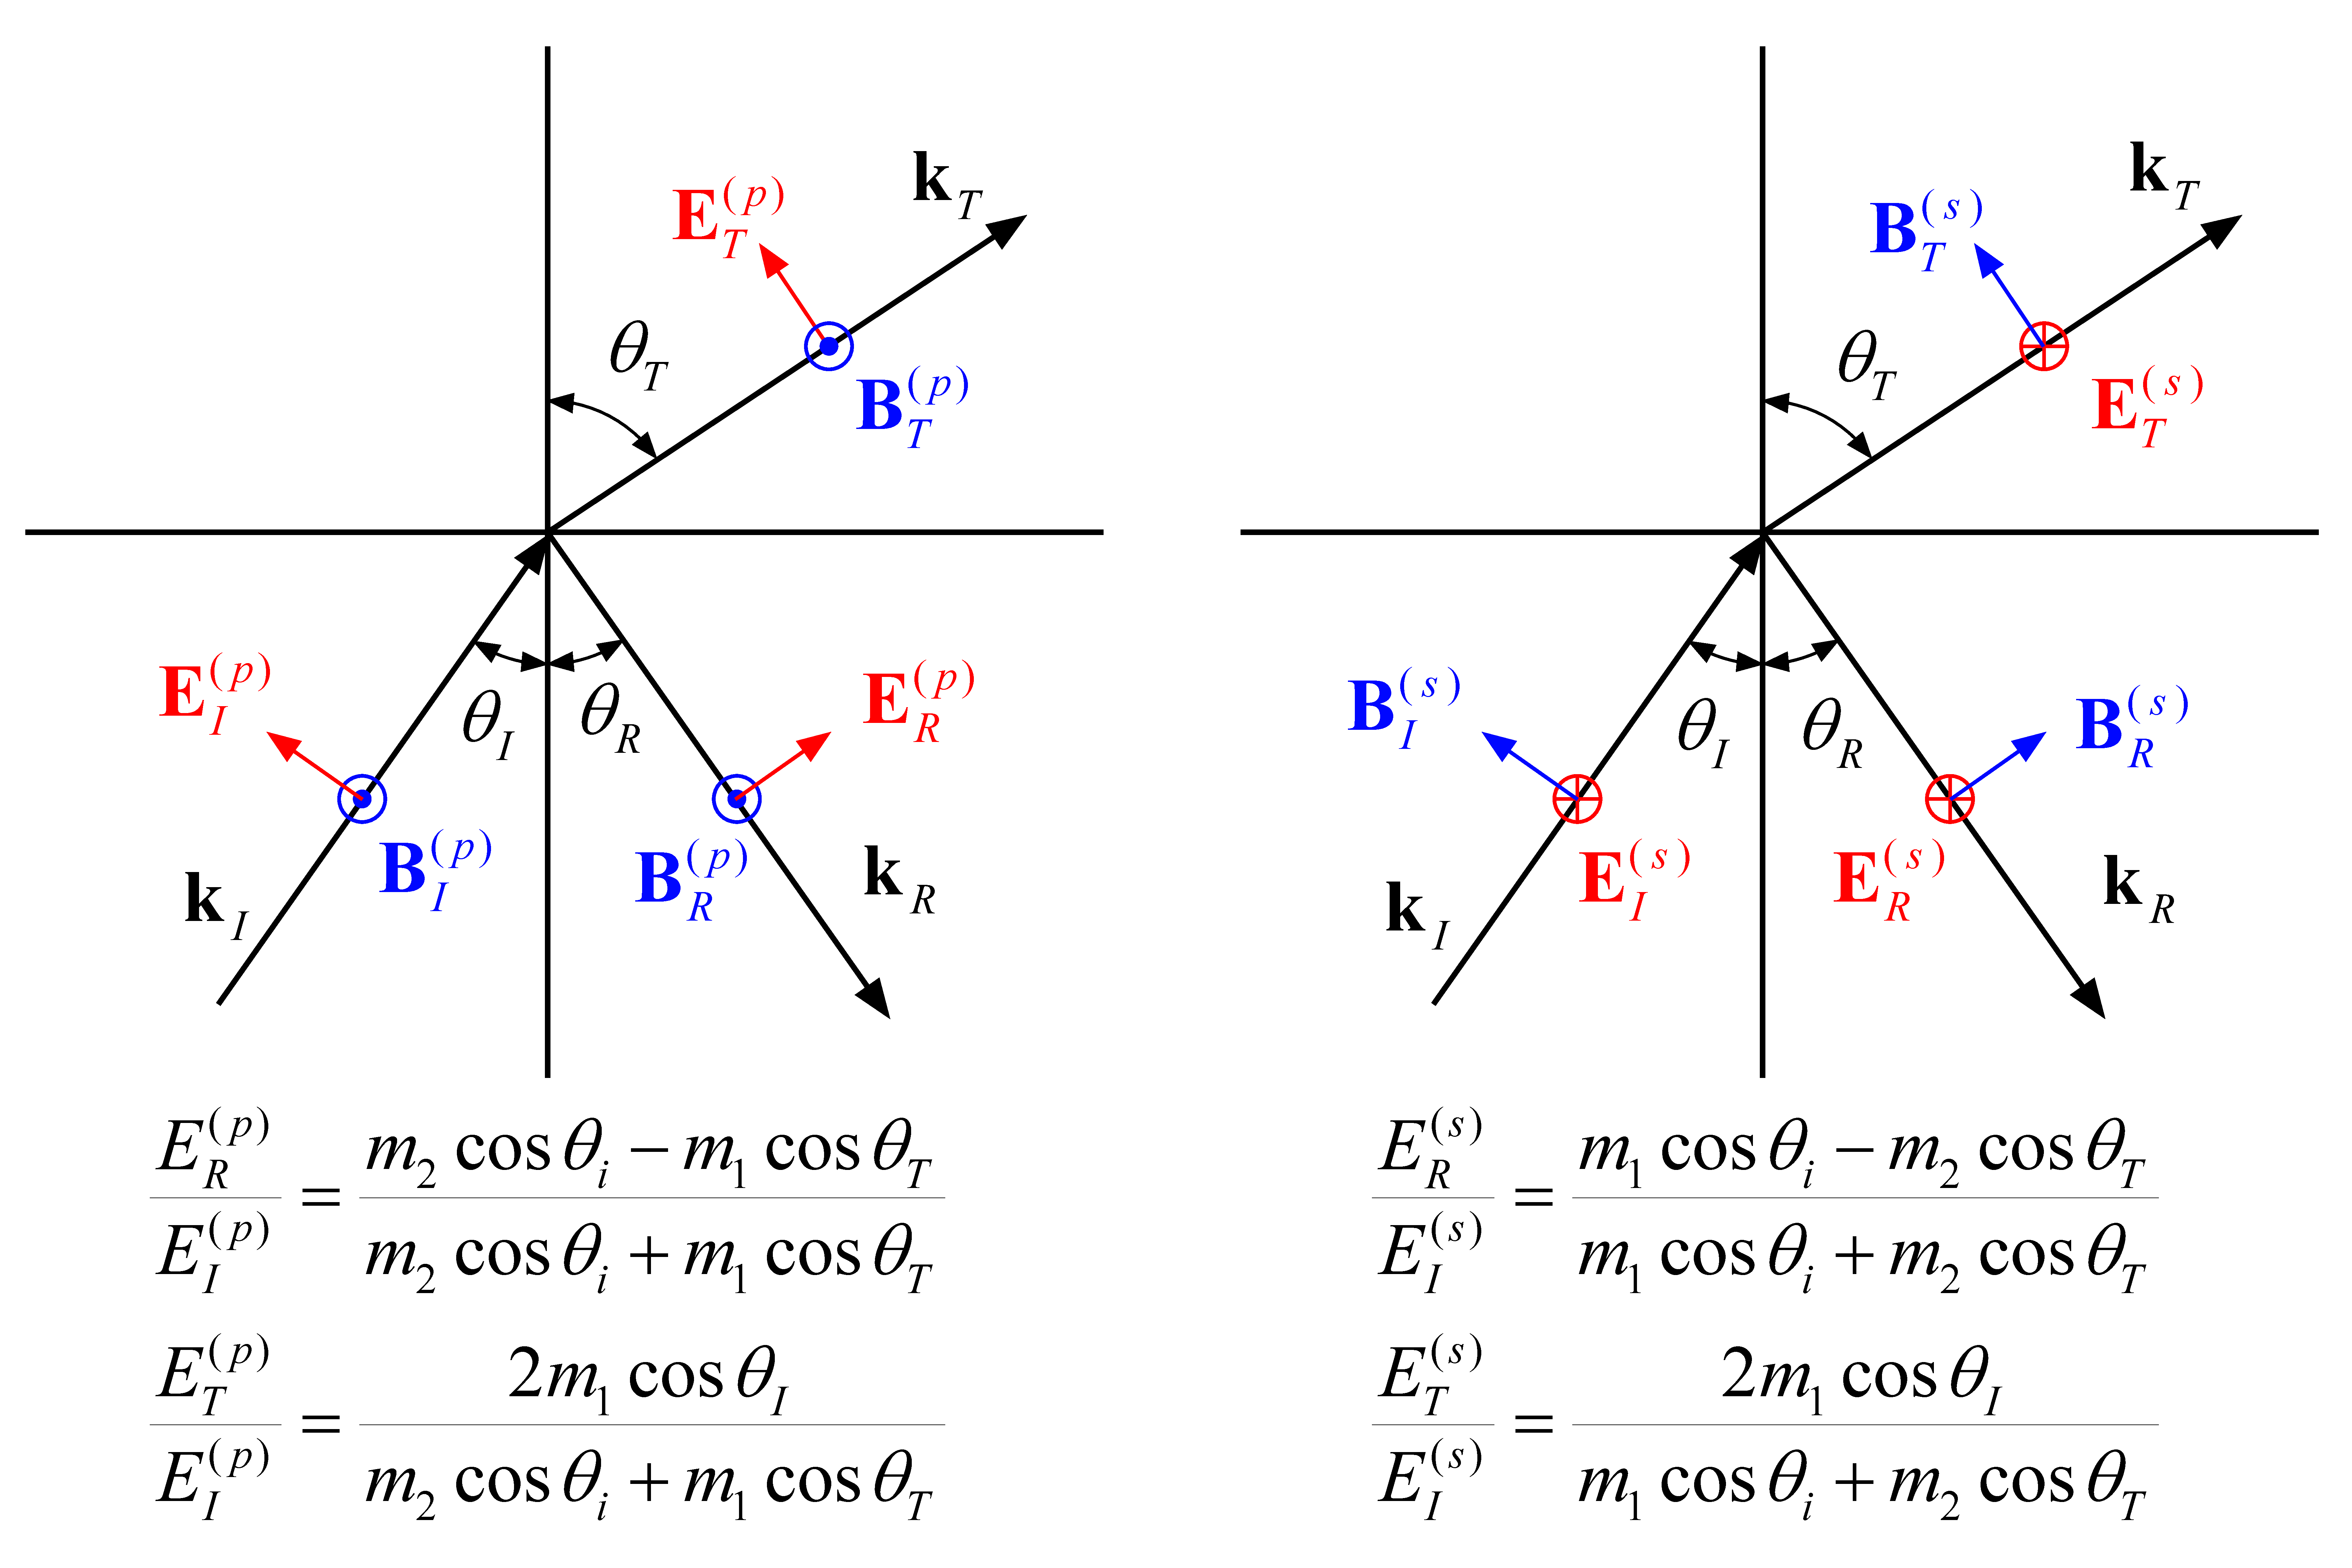
\includegraphics[width=14cm]{./figures/Fresnl.pdf}
\caption{菲涅尔公式} \label{Sample_fig1}
\end{figure}
 
利用具体的电磁场的边界条件 % 链接未完成
\begin{itemize}
\item $\div \vec D = 0$ 和$\div \vec B = 0$  分别对应 $\epsilon {\vec E_ \bot } = \epsilon '{\vec E'_ \bot }$; $\epsilon {\vec B_ \bot } = \epsilon '{\vec B'_ \bot }$ .

\item $\div \vec E = 0$ 和 $\div \vec H = 0$ 分别对应 ${\vec E_{//}} = {\vec E'_{//}}$ 和 ${{{{\vec B}_{//}}}}/{\mu } = {{{{\vec B'}_{//}}}}/{{\mu '}}$.
\end{itemize}

现在分两种情况讨论
\begin{enumerate}
\item 极化方向垂直于入射面 (右图)

\begin{equation}
\frac{{E_R^{(s)}}}{{E_I^{(s)}}} =  \frac{{{m_1}\cos {\theta _i} - {m_2}\cos {\theta _T}}}{{{m_1}\cos {\theta _i} + {m_2}\cos {\theta _T}}}
\qquad
\frac{{E_T^{(s)}}}{{E_I^{(s)}}} = \frac{{2{m_1}\cos {\theta _I}}}{{{m_1}\cos {\theta _i} + {m_2}\cos {\theta _T}}}
\end{equation}

\item 极化方向平行于入射面 (左图)
\begin{equation}\label{Fresnl_eq2}
\frac{{E_R^{(p)}}}{{E_I^{(p)}}} =  \frac{{{m_2}\cos {\theta _i} - {m_1}\cos {\theta _T}}}{{{m_2}\cos {\theta _i} + {m_1}\cos {\theta _T}}}
\qquad
\frac{{E_T^{(p)}}}{{E_I^{(p)}}} =  \frac{{2{m_1}\cos {\theta _I}}}{{{m_2}\cos {\theta _i} + {m_1}\cos {\theta _T}}}
\end{equation}
\end{enumerate}
其中 $m_i=n_i/\mu_i = c\sqrt{\epsilon_i/\mu_i}$, 一般情况下介质的磁导率于真空区磁导率的区别可忽略,即可以把 $m_i$ 替换为折射率 $n_i$. 另外注意菲涅尔公式包含相位信息,即以上的 $E$ 可以是复振幅.

\subsection{布儒斯特角}
我们这里考虑常见的 $n_2>n_1$ 且 $\mu_1=\mu_2$ 情况.由\autoref{Fresnl_eq2} 容易证明当入射角为\textbf{布儒斯特角(Brewster's angle)} 时反射光的平行(p)分量消失.布儒斯特角等于
\begin{equation}
{\theta _B} = \arctan ({n_2}/{n_1})
\end{equation}
% 未完成: 画图!